\section{Discoverable polynomial transport}\label{sec:discovery}
The central research object is the discovery of a transport representation.
A polynomial evaluated after its operator and degree have been supplied is
only the final stage. An accelerator must acquire the relevant coordinates,
relations, degree, and useful horizon from the available problem and current
state. Its cost includes that acquisition, unsuccessful candidates, and
verification. Structure in realistic data motivates this search; the
mathematical question is how that structure appears in the dynamics and
which part can be represented economically.

Every deterministic map already induces a linear transport on observables,
$(\mathcal U\phi)(z)=\phi(\F(z))$. This supplies an abstract sense in which
structure is transportable. Discovery asks for an economical finite portion
of that generally infinite function space, retaining the information that
determines the future state. A useful representation can be local in geometry
and horizon; it need not describe the entire problem with one fixed basis.

\subsection{From sparse coordinates to algebraic relations}
Tomi\'c, Widdershoven, and De Lathauwer encode $s$-sparsity by vanishing
products of $s+1$ distinct coordinates, combine these with the data equations,
and recover isolated solutions through structured null spaces and tensor
methods \cite{tomic}. Their Macaulay construction has combinatorial size;
their alternative optimization formulations use elementary symmetric
polynomials to evaluate sparsity expressions efficiently. This is a useful
algebraic perspective, not an iteration-acceleration theorem.

Our proposed connection is to discover relations among transported
observables, rather than assume that useful structure is sparse in the
original state coordinates. Several different notions must remain separate:
coordinate sparsity, small Krylov dimension, a sparse defining equation,
and finite-dimensional closure of observables. None implies all the others.
A sparse objective need not produce a low-degree iteration polynomial.

For an affine map, the ideal
\[
 \mathcal I_r=\{p\in\R[t]:p(J)r=0\}
\]
is generated by the relative minimal polynomial $\pi_r$. If its degree is
$s$, then every $p_m(J)r$ is represented by the remainder of $p_m$ modulo
$\pi_r$, of degree less than $s$. Arnoldi discovers this cyclic space by
operator actions; no eigenvalue list is required. In exact arithmetic,
closure after $s$ actions establishes this relation for that affine map.
For a self-adjoint propagator, $s$ counts distinct eigenvalues excited by
$r$, not the ambient dimension. Generalized eigenspaces and multiplicities
must also be retained for nonnormal maps.

A basis-independent analogue of sparsity is available for a data or
Krylov matrix $K$. Let $\lambda_i=\sigma_i(K)^2/\norm{K}_F^2$ for $K\ne0$,
ordered decreasingly, and let $e_j$ denote the elementary symmetric polynomial.
Then
\begin{equation}
 e_{s+1}(\lambda)=0\quad\Longleftrightarrow\quad\operatorname{rank}K\leq s.
 \label{eq:rankesp}
\end{equation}
Every summand is nonnegative, and a positive product of $s+1$ entries exists
exactly when at least that many singular values are nonzero. Moreover,
if $\lambda_s>0$,
\begin{equation}
 \sum_{i>s}\lambda_i
 \leq \frac{e_{s+1}(\lambda)}{\prod_{i=1}^{s}\lambda_i}. \label{eq:esptail}
\end{equation}
The numerator includes each product $\lambda_1\cdots\lambda_s\lambda_i$
for $i>s$. The denominator explains why a small vanishing-relation residual
alone is not a conditioning-independent approximate-rank certificate.
The elementary recurrence evaluates $e_{s+1}$ in $O(ns)$ operations once
its arguments are available; acquiring singular information is not free.
We test this identity as a diagnostic, not as a promoted rank-selection rule.

\subsection{Closure of observables is stronger than tangent closure}
Suppose a lift $\Phi:\Omega\to\R^d$ contains enough information to recover
the state through $z=C\Phi(z)$, and
\begin{equation}
 \Phi(\F(z))=T\Phi(z),\qquad z\in\Omega,\quad \F(\Omega)\subseteq\Omega.
 \label{eq:liftclosure}
\end{equation}
Then $\F^m(z)=CT^m\Phi(z)$. This follows by induction and is a standard
finite-dimensional Koopman representation; discovering such observable
spaces has substantial prior literature \cite{brunton,ssd}. Cayley--Hamilton
reduces every $T^m$ modulo its minimal polynomial. The useful discovery is
therefore the representation and its validity, not merely the exponentiation.
For approximate closure
$\Phi(\F(z))=T\Phi(z)+\eta(z)$ with exact decoder $C$, the error identity is
\begin{equation}
 \F^m(z)-CT^m\Phi(z)
 =\sum_{j=0}^{m-1}CT^{m-1-j}\eta(\F^j(z)).
 \label{eq:liftdefect}
\end{equation}
This follows by telescoping the lifted recurrence. It shows why discovery
must control both closure error and its amplification; a small fitted
residual by itself is not a long-horizon prediction guarantee.

For a concrete checked control, consider
\[
 u^+=a u,\qquad v^+=b v+c u^2,\qquad
 \Phi(u,v)=(1,u,v,u^2)^T.
\]
The lift obeys \eqref{eq:liftclosure} with
\[
 T=\begin{pmatrix}
 1&0&0&0\\0&a&0&0\\0&0&b&c\\0&0&0&a^2
 \end{pmatrix}.
\]
The coefficients of $T$ can be identified from full-row-rank lifted probe
matrices. Independent probes verify the recovered identity in the control.
The two-dimensional state Jacobian already has a closed Krylov space, yet
its frozen long-horizon trajectory is wrong because $u^2$ evolves. This
example is a representation control, not a claimed mirror-descent model
or a new Koopman algorithm.

There is a finite verification theorem when the function class is known.
If every component of $\Phi\circ\F-T\Phi$ lies in a specified polynomial
space $\mathcal P$, and evaluations at the chosen probes are injective on
$\mathcal P$, zero residual at those probes proves the identity throughout
the domain. Indeed, the only member of $\mathcal P$ vanishing on an
unisolvent set is zero. Without a degree or function-class constraint,
finite probes provide no such proof: a perturbation supported away from
all queried points can alter an unqueried future state.

Polynomial relations among observables may reduce a dictionary through an
invariant ideal, but that does not automatically leave a finite-dimensional
observable space. A polynomial coordinate algebra on a continuous state
set is generally infinite-dimensional. The finite-root quotient in sparse
recovery and the invariant observable space needed here are related
algebraic tools, not interchangeable assumptions.

\subsection{An acquisition screen and its informative failure}
We implemented incremental Arnoldi depths $2,4,8,12$, testing horizons
$64,32,16,8$. A candidate is screened at its quarter, half, and penultimate
predicted states with actual map calls. Its score is the horizon times the
largest sampled defect, divided by predicted displacement. The threshold
is $0.05$ and nominal saved work must exceed total acquisition and settling
work by a factor of $1.5$. These are fixed exploratory choices. Sparse
samples falsify candidates; they do not bound defects at unqueried states.

The retained screen has 66 anchors across two seeds, four spectral-degree
controls, entropy simplex, three ADMM penalties, and camera/Barbara Meyer
maps with histogram-preserving spatial permutations. It accepts 35 anchors;
the largest independently measured relative trajectory error among those
accepted is $0.0200$. At the early anchors of the two-, four-, and eight-mode
controls, the discovered depths are respectively two, four, and eight.
The coefficients and spectral labels are withheld from the scanner.
Later anchors often need less depth because fast modes have decayed.

The same rule rejects every natural and permuted Meyer anchor. At a
512-work-unit budget it also spends substantial effort rejecting candidates
in restarted solves. This is not evidence against the existing Meyer
accelerator: its fixed finite proposals can improve the objective while
having substantial error relative to the ordinary trajectory. For camera
at prefix four, the depth-four/horizon-sixteen relative trajectory error is
$0.585$, yet the fixed accelerated solve improves the final certified gap
relative to ordinary iteration at the same work budget. A requirement to
reproduce the whole ordinary path accurately is therefore sufficient for
some acceleration arguments, but is not necessary for useful acceleration.
The sampled screen is retained as a diagnostic and is not promoted as the
new general method.

\subsection{Certified discovery on affine pieces of a convex mirror map}
A class with stronger available structure permits actual certification.
Consider the Huber inverse problem
\[
 f(x)=\sum_i h_\delta((Ax-b)_i),\qquad
 \psi(x)=\tfrac12 x^TGx,\quad G\succ0,
\]
where $h_\delta'(a)=\operatorname{clip}(a,-\delta,\delta)$.
In whitened dual coordinates $t=G^{1/2}x$, put $B=AG^{-1/2}$. The map is
\begin{equation}
 \F(t)=t-\alpha B^T\operatorname{clip}(Bt-b,-\delta,\delta),
 \qquad 0<\alpha\leq 2/\norm{B}_2^2. \label{eq:huber}
\end{equation}
It is globally nonexpansive in Euclidean $t$-norm: the difference of two
updates is $(I-\alpha\overline B)(t-s)$, where the averaged Hessian obeys
$0\preceq\overline B\preceq\norm{B}_2^2 I$. Hence the eigenvalues of the
difference operator lie in $[-1,1]$. Fix an anchor $t$, residual $a=Bt-b$, and mask
$D_{ii}=1_{\{|a_i|<\delta\}}$. On the corresponding closed affine piece,
\[
 J=I-\alpha B^TDB,\qquad
 \F(t+v)=\F(t)+Jv.
\]
The projected path is $\widehat t_j=t+Qc_j$, where
$c_0=0$ and $c_{j+1}=\beta e_1+Hc_j$.
Every piece constraint can be checked using only
\begin{equation}
 a_j=a+(BQ)c_j. \label{eq:featurepath}
\end{equation}
The columns $Bq_i$ are already computed by the tangent actions and cached.
The checks require feature-space operations, not another $B^T$ application
or another full map. Their execution time is nevertheless charged.

\begin{theorem}[An affine-piece discovery certificate]\label{thm:piece}
If \eqref{eq:featurepath} remains in the anchor's closed piece for every
input index $j=0,\ldots,m-1$, and $E=JQ-QH$, then
\begin{equation}
 \norm{\F^m(t)-(t+Qc_m)}_2
 \leq \sum_{j=0}^{m-1}\norm{Ec_j}_2. \label{eq:piecebound}
\end{equation}
In particular, algebraic closure $E=0$ makes the discovered finite
transport exact, even when its final output crosses a piece boundary.
\end{theorem}
\begin{proof}
The checked affine formula gives
$\F(\widehat t_j)-\widehat t_{j+1}=Ec_j$ at every predicted input.
For the actual state $t_j$, nonexpansivity gives
$\norm{t_{j+1}-\widehat t_{j+1}}
\leq\norm{t_j-\widehat t_j}+\norm{Ec_j}$.
Induction proves the bound. It is not necessary to assume that the
unknown actual path stays inside the same piece. The last checked point
is input $m-1$, not output $m$.
\end{proof}

The norms in \eqref{eq:piecebound} use the small Gram matrix $E^TE$.
This gives a computable path certificate in exact arithmetic and a
floating-point diagnostic with explicit numerical tolerance in the code;
we do not claim directed-rounding certification. An exterior Euclidean
disk projection is curved, so this theorem does not transfer to Meyer
merely because its inside/outside mask stays unchanged.

\subsection{Unit-mode drift and the Anderson distinction}
If all Huber residuals are saturated, then $D=0$, $J=I$, and
$r=-\alpha B^T\operatorname{sign}(a)\delta$ is constant until the next event.
The first Arnoldi action discovers a rank-one cyclic space, and
$p_m(J)r=mr$. Put $d=Br$. For every feature moving toward its nearest
boundary, the continuous crossing time is
\[
 \tau_i=\frac{\operatorname{sign}(a_i)\delta-a_i}{d_i}>0.
\]
The horizon $m=1+\lfloor\min_i\tau_i\rfloor$ has all inputs in the current
closed piece and may place its output beyond the first boundary. A finite
cap limits acquisition amortization; endpoint roundoff is checked in code.
Thus the drift direction, one-dimensional relation, and first-event horizon
are all obtained from the current problem. They are not supplied by a
known optimum or by a future reference trajectory.

For type-II Anderson using a history entirely within this same constant-drift
piece, every residual difference is zero. With the minimum-norm or positive
ridge least-squares convention, its extrapolation coefficients are zero:
it takes one ordinary step. This is a precise collapse of acceleration,
not divergence of the underlying iteration. More generally, a left invariant direction $w^TJ=w^T$ with $w^Tr\ne0$
obstructs a stationary correction because $w^T(I-J)\delta=0$, while
$w^Tp_m(J)r=mw^Tr$ retains the required drift. This is the same structural
question raised by the earlier Meyer chart audit: a locally persistent
pattern can carry an unresolved future event. History spanning other pieces,
roundoff, or alternative regularization can change the behavior; no universal
Anderson failure is asserted. The earlier coupled Meyer/subproblem stall,
the later full-state synthetic comparisons, and this exact drift mechanism
must remain distinct pieces of evidence.

\subsection{Camera-derived inverse problems and complete cost}

The Huber study uses a camera image resized to $8\times8$ or $16\times16$, with $n=64$ or $256$ unknowns and $4n$ synthetic measurements. The sensing matrix has independent Gaussian entries scaled by $1/\sqrt{4n}$; the positive variant takes their absolute values. The mirror diagonal spans $[1,16]$. Observations are noiseless, $b=Ax_*$, so the minimum objective is zero. These are controlled camera-derived inverse problems, not a benchmark of naturally corrupted measurements. Both sensing variants are retained.

The first positive-sensing blocks at $n=64$ discover horizons $392$, $366$, and $386$ on the three seeds. Each uses one map and one tangent action. Independent replay disagrees by at most $8.6\times10^{-12}$ in absolute whitened dual norm. At $n=256$, the corresponding discovered horizons are $838$, $831$, and $821$, with maximum absolute replay error $3.7\times10^{-11}$. These are exact-arithmetic drift skips verified numerically; the long horizon is determined by the first feature event.

For the complete solve, the certified method tries depths $2,4,8$, caps horizons at $4096$, and requires the bound in \eqref{eq:piecebound} to be at most $0.02\norm{Qc_m}$. It takes sixteen ordinary steps after an unprofitable acquisition. The target is an objective-gap ratio of $10^{-3}$, checked every sixteen work units. Three seeds and three shuffled timing repeats per seed are used on the M4 Mini with one BLAS thread. Timings include discovery, boundary checks, unsuccessful attempts, and objective checks, but exclude matrix setup. All methods reach the target on all seeds in this study.

\begin{table}[htbp]\centering\small

\begin{tabular}{lr rrrr}\toprule

Sensing & $n$ & Ordinary & Fixed & Discovered & Anderson\\\midrule

Positive & 64 & 94.26 & 73.50 & 104.73 & 21.87\\

Signed & 64 & 8.67 & 7.05 & 48.77 & 5.10\\

Positive & 256 & 3002.11 & 1218.88 & 878.85 & 135.01\\

Signed & 256 & 72.87 & 30.48 & 155.87 & 14.45\\

\bottomrule\end{tabular}

\caption{Complete solve milliseconds, median of the per-seed timing medians. Fixed means depth four/horizon sixteen with one settling step. Discovered means the affine-piece certificate.}

\label{tab:discovery}\end{table}

At $n=256$ with positive sensing, the discovered method is 3.47$\times$ faster than ordinary iteration and 1.42$\times$ faster than the fixed finite schedule, using paired per-seed median time ratios. At $n=64$ its acquisition overhead prevents an overall speedup. On signed sensing, frequent piece events make this certificate costly and the discovered method is slower at both sizes. Anderson wins the complete solves here after the initial constant-drift phase ends. The proved local drift obstruction therefore does not imply an end-to-end ranking.

The full solve also exposes a stability distinction hidden by final runtime alone. On positive-sensing seeds zero and one at $n=256$, Anderson reaches recorded objective gaps $25.26$ and $7.35$ times the initial gap before recovering. The certified transport has no comparable excursion at the recorded checkpoints. Checks occur every sixteen work units, so this is not a bound on all intermediate gaps or a claim of monotonicity for approximate certified proposals.

Measurements from the initial scalar implementation of the reduced-path checks are retained as protocol v1. Protocol v2 uses block doubling for $c_j$ and batched feature tests without changing mathematical admission conditions. Both raw records remain available; v2 is used in Table~\ref{tab:discovery}.

\begin{figure}[htbp]\centering

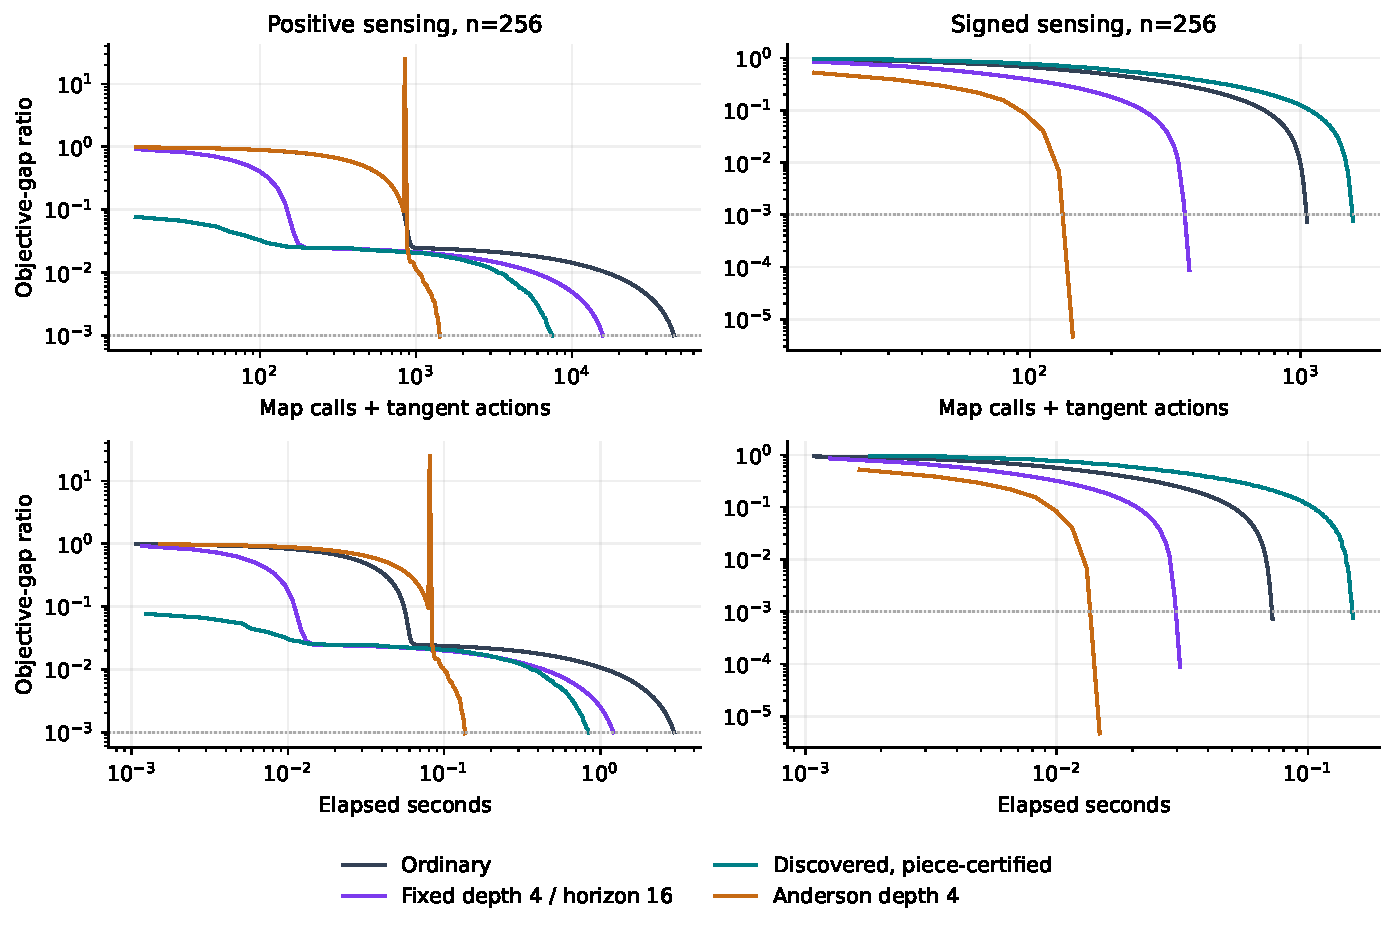
\includegraphics[width=\textwidth]{figures/discovery_costs.pdf}

\caption{Huber mirror descent at $n=256$, seed zero, first timed repeat. The same camera source and target tolerance are used for positive and signed sensing. A discovered valid polynomial can save work and time, while frequent boundary changes can eliminate that benefit. The timing table retains all seeds and repeats.}

\end{figure}

This extension establishes a discoverable, checkable finite transport construction for a nontrivial convex mirror class. The central unresolved problem is to discover comparably economical validity descriptions for curved proximal geometry and changing observable spaces, including the original coupled Meyer iteration.

